% Committee progress update, 23 September 2026 -- the single bound submission.
%
% This document writes no new prose. It binds four existing PDFs, each of which
% keeps the job it was written for, behind a cover and a one-page reading guide:
%
%   summary.pdf    2 pp   executive summary, reads cold without the rest
%   main.pdf      68 pp   the full record, with repository evidence
%   concerns.pdf   7 pp   every queried passage, as a checklist
%
% The slides are deliberately NOT bound in: they are for presenting, not reading,
% and their content is a subset of the summary.
%
% Why bind rather than merge into one rewritten document: the report's register
% -- repository paths, anomaly keys, run identifiers -- is what makes its
% implementation claims checkable, and is required of it. Rewriting that register
% for a committee audience would destroy the evidence base to gain a readability
% the summary already provides. Binding gives one artifact to hand over while
% each part keeps doing its own job.
%
% Rebuild: compile the three sources first, then
%   latexmk -pdf docs/report/committee_20260923/progress_update.tex

\documentclass[11pt,a4paper]{article}

\usepackage[T1]{fontenc}
\usepackage[utf8]{inputenc}
\usepackage{lmodern}
\usepackage[margin=24mm]{geometry}
\usepackage{microtype}
\usepackage{xcolor}
\usepackage{enumitem}
\usepackage{pdfpages}
\usepackage[hidelinks]{hyperref}

\definecolor{flagred}{HTML}{B00000}
\newcommand{\flag}[1]{\textcolor{flagred}{#1}}
\setlist{nosep}
\pagestyle{empty}

\hypersetup{
  pdftitle={WiL Committee Progress Update},
  pdfauthor={Bolton Athit Davies}}

\begin{document}

% ---------------------------------------------------------------- cover
\vspace*{0.22\textheight}
\begin{center}
  {\Huge\bfseries Vision-Based Navigation\\[0.35em] for AMRs in a Dynamic
   Warehouse}\\[2.2em]
  {\LARGE Committee progress update}\\[2.8em]
  {\large Bolton Athit Davies}\\[0.9em]
  {\large 23 September 2026}\\[2.6em]
  {\normalsize Reporting cutoff 16 September 2026,\\[0.3em]
  with three later additions marked where they appear}
\end{center}
\vfill
\begin{center}
  \small
  Executive summary (2\,pp) \quad$\cdot$\quad Progress report (68\,pp)
  \quad$\cdot$\quad Open concerns (7\,pp)
\end{center}
\clearpage

% ---------------------------------------------------------------- reading guide
\section*{How to read this document}

Three documents are bound here. They are written for different readers and are
meant to be used differently.

\subsection*{1. Executive summary --- 2 pages}

Written to be read cold, without the rest and without prior knowledge of the
project. It states the research question, what is established, what is not, and
what guidance is requested. \textbf{If you read only one part, read this one.}

\subsection*{2. Progress report --- 68 pages}

The full record, and the evidence behind every number in the summary. Its
register is deliberately technical: implementation claims cite the exact source
file, configuration key, run identifier or commit that supports them, so that any
claim can be checked rather than taken on trust. It is not written to be read
straight through. Use the table of contents, or follow a reference from the
summary.

\subsection*{3. Open concerns --- 7 pages}

Every passage the report marks as \flag{queried}, collected into one checklist of
67 items. This is the fastest route to ``what does the author not yet stand
behind?''

\bigskip
\hrule
\bigskip

\subsection*{What the red text means}

A red passage marks a result, number or condition that is \emph{measured but not
yet trustworthy as evidence} --- an unexplained mechanism, a confound, an unfair
comparison, or a figure whose provenance does not support the use it is being put
to.

It deliberately does \textbf{not} mark a bad result. A large error that is
correctly measured and understood is a finding, and appears in black. The red
marks doubt about the evidence, not disappointment with the outcome. Sixty-seven
such passages is a consequence of flagging aggressively, not of the work being
unusually uncertain.

\subsection*{What is deliberately excluded}

Trajectory results from the dynamic-scene recordings are withheld. Those worlds
move their props along scripted kinematic paths: the props carry collision
geometry but produce no dynamic response against the robot, and nothing
constrains them to behave as warehouse traffic would. Forty-eight runs were
logged there and all forty-eight fail a physical-plausibility check, but those
numbers describe the simulation rather than the problem, so they are retained in
the report as excluded evidence rather than reported as findings.

The consequence is stated plainly in both the summary and the report: the
condition this work is named for currently has no valid testbed. It is untested,
rather than tested and failed, and rebuilding those worlds is the first item of
the next period.

\subsection*{A note on the reporting cutoff}

The report's cutoff is 16 September 2026, and components are labelled
\emph{implemented}, \emph{verified}, \emph{partially verified}, \emph{blocked},
\emph{failed} or \emph{planned} as at that date. Three pieces of work landed
after it and are marked as later additions in the text rather than folded in
silently: relative pose error, the dense-map evaluation, and the
simulation-fidelity assessment. The cutoff was left where it was precisely so
that those additions stay visible as additions.

\clearpage

% ---------------------------------------------------------------- bound parts
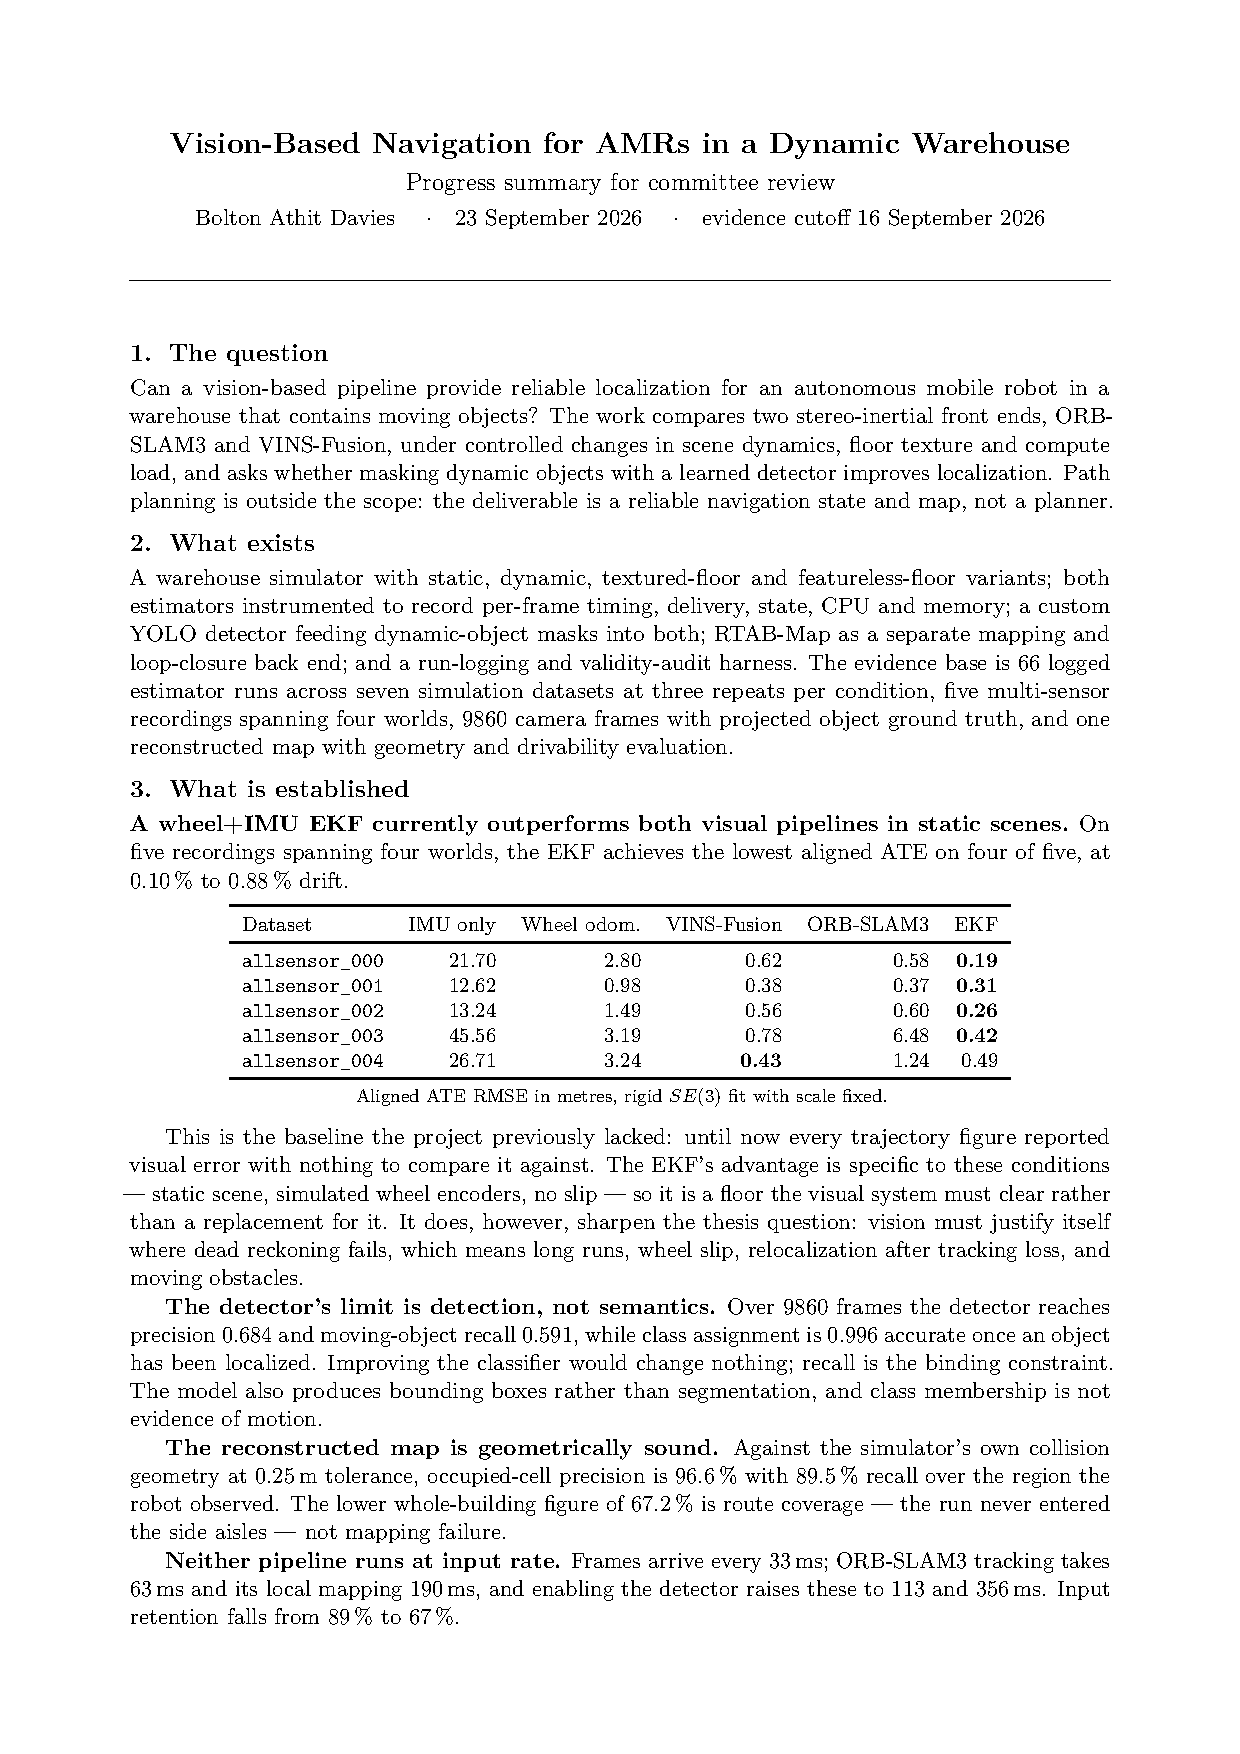
\includepdf[pages=-]{summary.pdf}
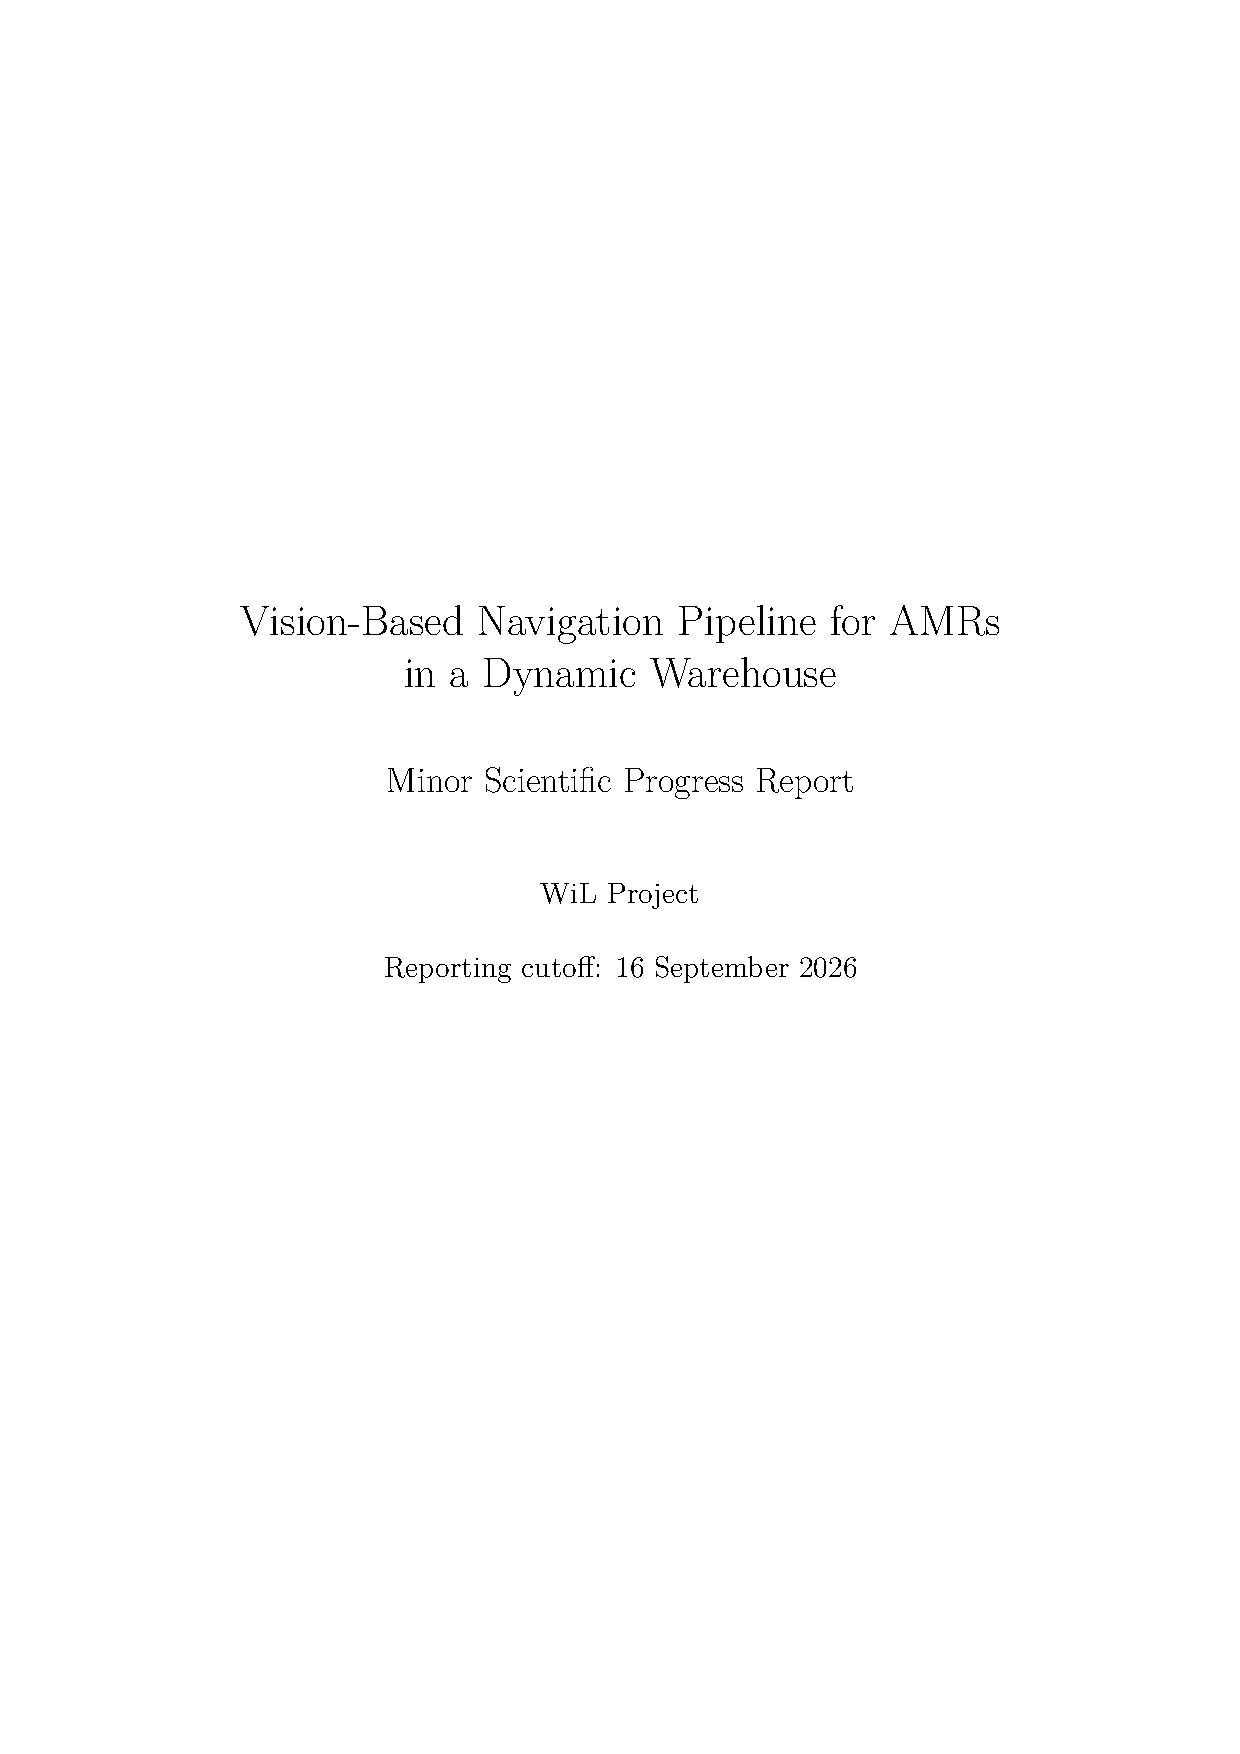
\includepdf[pages=-]{../minor_report/main.pdf}
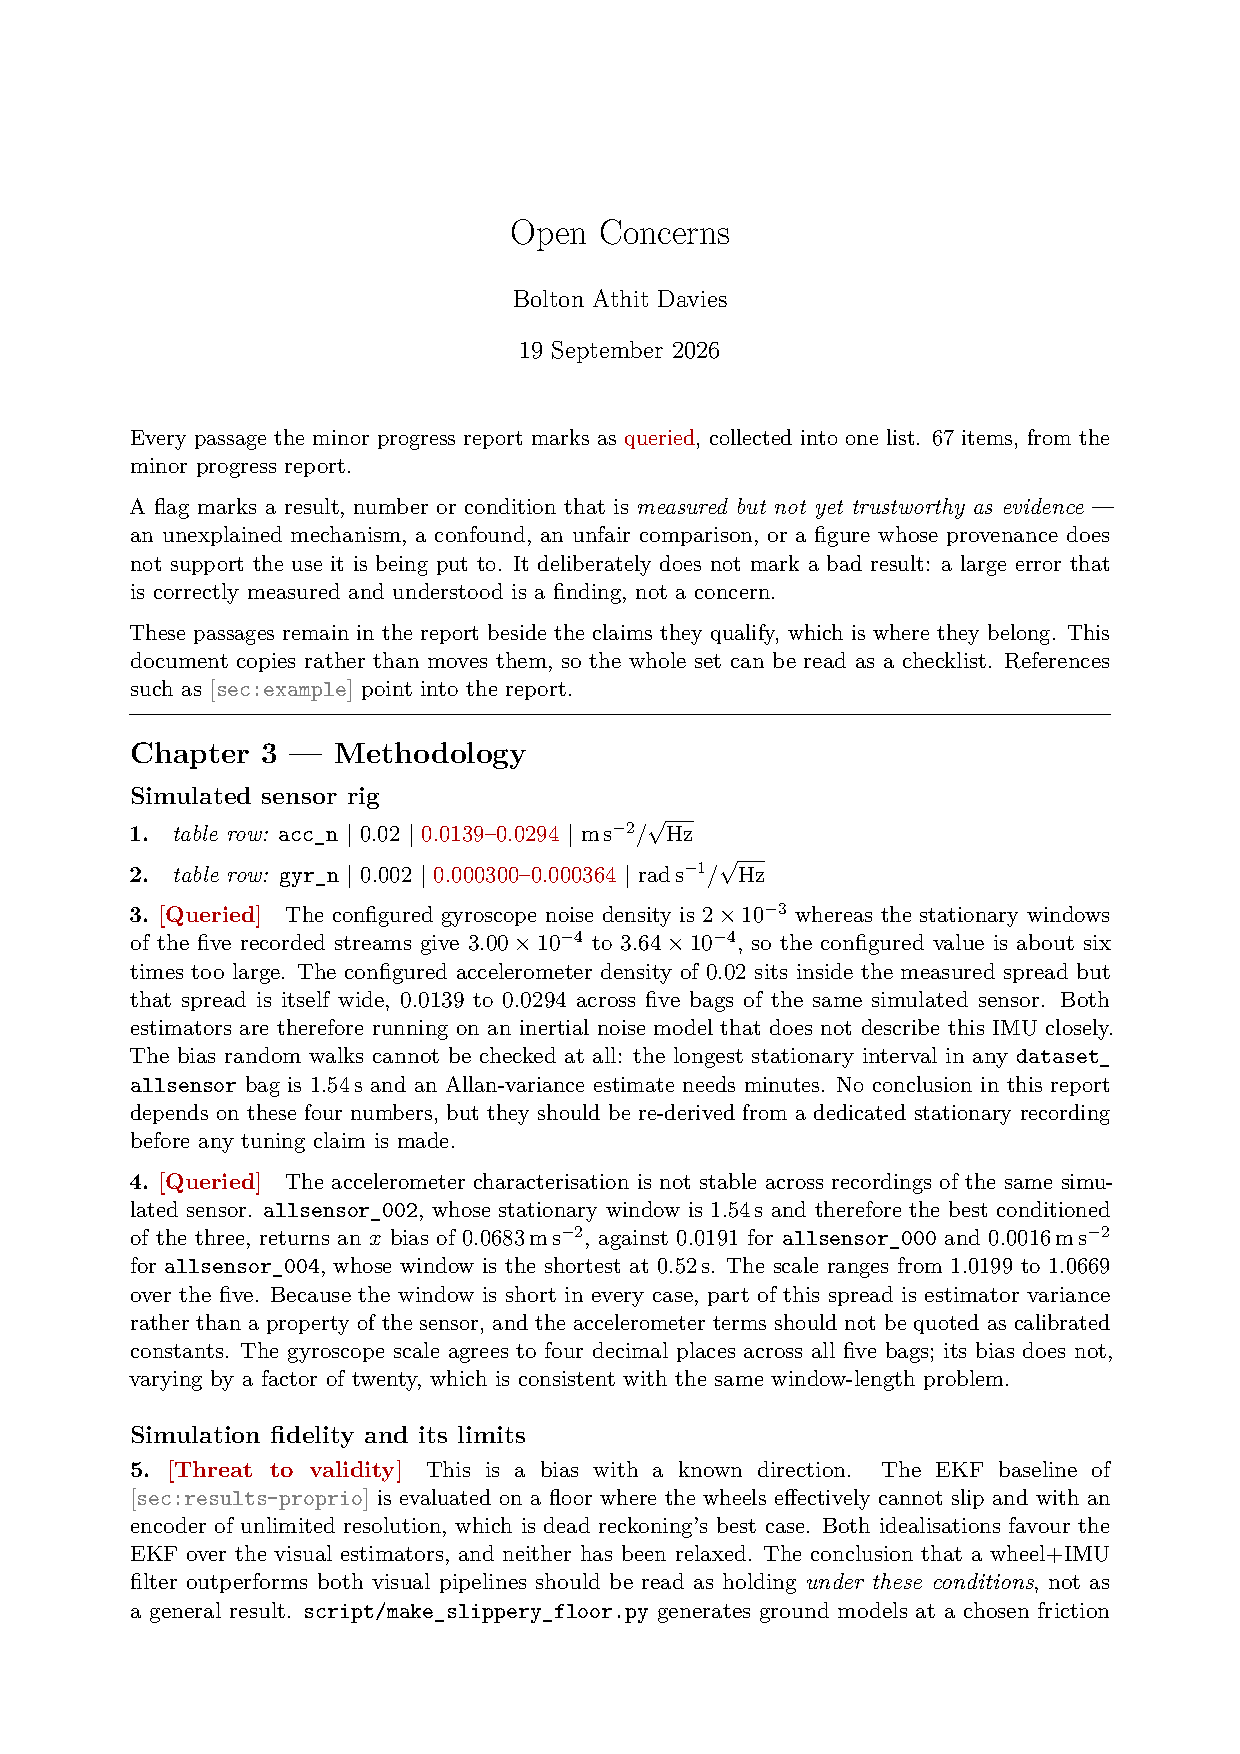
\includepdf[pages=-]{../concerns/concerns.pdf}

\end{document}
